\documentclass[11pt]{article}
\usepackage{latexsym}
\usepackage{amsmath}
\usepackage{amssymb}
\usepackage{amsthm}
\usepackage{epsfig}
\usepackage[tight]{subfigure}
\usepackage{caption}
\usepackage{booktabs}
\usepackage{graphicx}

\DeclareMathOperator*{\minimize}{min}
\DeclareMathOperator*{\maximize}{max}

\usepackage{algorithm}
 %on linux you may need to run sudo apt-get install texlive-full to install algorithm.sys
\usepackage{algorithmic}

\usepackage{verbatim}
\usepackage{listings}
\usepackage{xcolor}
\lstset{
    basicstyle=\small\ttfamily,
    backgroundcolor=\color{gray!10},
    frame=single,
    framerule=0pt,
    escapeinside={(*@}{@*)},
    breaklines=true,
    columns=fullflexible,
    keepspaces=true,
}

\newcommand{\handout}[6]{
  \noindent
  \begin{center}
  \framebox{
    \vbox{
      \hbox to 5.78in { {#1} \hfill #2 }
      \vspace{4mm}
      \hbox to 5.78in { {\Large \hfill #5  \hfill} }
      \vspace{1mm}
      \hbox to 5.78in { {\Large \hfill #6  \hfill} }
      \vspace{2mm}
      \hbox to 5.78in { {\em #3 \hfill #4} }
    }
  }
  \end{center}
  \vspace*{4mm}
}

\newcommand{\lecture}[6]{\handout{#1}{#2}{#3}{#4}{#5}{#6}}
\newcommand{\collision}[0]{\mathrm{collision}}
\newcommand{\nocollision}[0]{\overline{\collision}}

\newcommand*{\QED}{\hfill\ensuremath{\square}}

\newtheorem{theorem}{Theorem}
\newtheorem{corollary}[theorem]{Corollary}
\newtheorem{lemma}[theorem]{Lemma}
\newtheorem{observation}[theorem]{Observation}
\newtheorem{proposition}[theorem]{Proposition}
\newtheorem{definition}[theorem]{Definition}
\newtheorem{claim}[theorem]{Claim}
\newtheorem{fact}[theorem]{Fact}
\newtheorem{assumption}[theorem]{Assumption}
\newtheorem{note}[theorem]{Note}

% 1-inch margins, from fullpage.sty by H.Partl, Version 2, Dec. 15, 1988.
\topmargin 0pt
\advance \topmargin by -\headheight
\advance \topmargin by -\headsep
\textheight 8.9in
\oddsidemargin 0pt
\evensidemargin \oddsidemargin
\marginparwidth 0.5in
\textwidth 6.5in

\parindent 0in
\parskip 1.5ex

\title
{ 
{\small Multi Robot Planning and Coordination (16-891) Spring 2026 - The Robotics Institute} \\
Homework 2 : Multi-Agent Path Finding (MAPF) \\
{\small Instructor: Jiaoyang Li \;\;\; TA: Philip Huang, Jingtian Yan }\\
}
\author{Ranai Srivastav}

\begin{document}

\maketitle

\textbf{Collaborators:}
%Everyone you collaborated with and a short description of what you discussed.
\begin{enumerate}
    \item Tom Gao - Discussed problems, brainstormed edge cases
    \item Claude  - Took help with understanding algorithms, format latex.
                    All code, answers to theory questions, and analysis is written by me.
\end{enumerate}

\section*{Task 1 - Included Code}

\section*{Task 2 - Is there a need to find edge constraints when k $\geq$ 1}
    \textbf{No, there is no need to find edge constraints when k is larger than 0.} \\
    Let's assume two agents, A and B, where A is at P and B is at Q at time t.
    By definition, an edge conflict will occur when A tries to go to Q and B tries to go to P at time t+1.
    Both P and Q are in the trajectories of each of the agents and since A and B can go from P to Q or vice versa in one timestep, P and Q must be neighbors.

    Now there are two cases:
    \begin{enumerate}
        \item Agent A waits at current state for some non-zero number of steps, in which case an edge conflict cannot occur, only a vertex constraint. Thus, P and Q cannot be the same state.
        \item Agent A has moved at timestep t.
        For an edge conflict to occur, the next step for both agents must be within reach in one timestep.
        This is only possible if both agents are in each other's 1-action neigborhood, which implies that any locations farther than the 1-action neighborhood do not need to be checked.
        In other words, since the robots need to exchange positions along the same edge for an edge conflict, and agents cannot teleport, the states can only be one timestep away, exactly.
    \end{enumerate}

    Running KR-CBS with k=0 in a realistic setting would mean that we are very sure of each robot's execution and pose at all times.
    This is an unrealisitic assumption and even if execution is not an issue, planning a path like this would mean robots will be too close to each other.
    If in a hierarchical planning framework, this would mean that the local agent-level trajectory follower will have to replan whenever the speed assumptions are violated.


\section*{Task 3 - Included Code}
\section*{Task 4 - Running Statistics}

    \begin{table}[h]
  \centering
  \begin{tabular}{|l|c|c|c|c|}
  \hline
  \textbf{Map Name} & \textbf{CPU Time (s)} & \textbf{Sum of Costs} & \textbf{Num Expanded} & \textbf{Generated Nodes} \\
  \hline
  instances/test\_1.txt & 0.00 & 24 & 4  & 7   \\
  instances/test\_1.txt & 0.11 & 28 & 78 & 155 \\
  instances/test\_1.txt & 0.01 & 22 & 5  & 9   \\
  instances/test\_1.txt & 0.04 & 26 & 29 & 57  \\
  instances/test\_1.txt & 0.01 & 26 & 7  & 13  \\
  instances/test\_1.txt & 0.01 & 26 & 7  & 13  \\
  instances/test\_1.txt & 0.00 & 20 & 4  & 7   \\
  instances/test\_1.txt & 0.00 & 24 & 2  & 3   \\
  instances/test\_1.txt & 0.11 & 32 & 82 & 163 \\
  instances/test\_1.txt & 0.00 & 28 & 2  & 3   \\
  instances/test\_1.txt & 0.00 & 18 & 2  & 3   \\
  instances/test\_1.txt & 0.01 & 28 & 8  & 15  \\
  \hline
  \end{tabular}
  \caption{TA-Random results on instances/test\_1.txt ($k=2$, 12 samples)}
  \label{tab:ta_random_stats}
  \end{table}

  \noindent\textbf{Stats on sum of costs (12 samples):}\\
  \textbf{
    Min = 18
    Max = 32
    Mean = 25.16,\
    Std.\ Dev.\ = 3.69,\
    Variance $\approx$ 13.61}

  \medskip
  \noindent\textbf{Stats on number of generated nodes (12 samples):}\\
  \textbf{
      Min = 3
      Max = 163
      Mean = 37.33,\
      Std.\ Dev.\ = 56.18,\
      Variance $\approx$ 3156.19}
    
\section*{Task 5 - Included Code}

\section*{Task 6 - Stats for TA-Distance}
CPU time (s):    0.02
Sum of costs:    16
Expanded nodes:  3
Generated nodes: 5
The sum of costs is smaller for TA-DISTANCE and so is the number of generated nodes.
The sum of the lengths of the paths of each agent is smaller than TA-DISTANCE and because TA-DISTANCE uses the hungarian algorithm which gaurantees the
optimal solution, this cost is the lowest possible cost achievable in this map given that any of the limitations of hungarian algorithm are not met such as a changing map.

\section*{Task 7}
\begin{figure}[H]
    \centering
    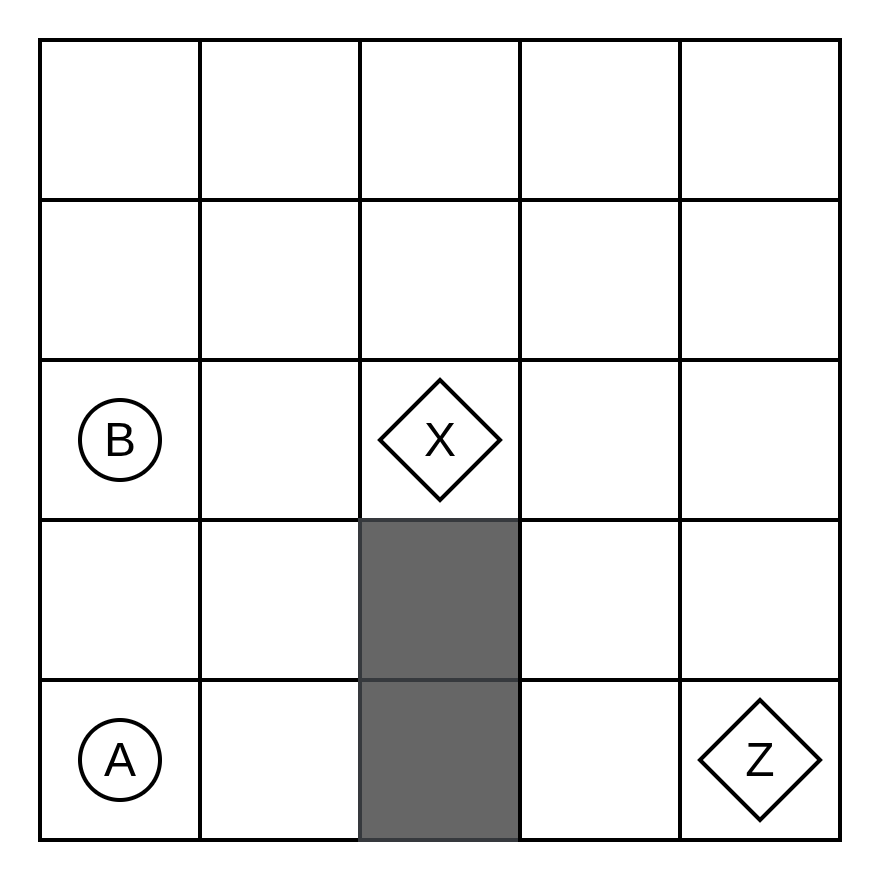
\includegraphics[scale=0.5]{images/unoptimal}
    \caption{Assigning tasks once cannot take into account changing cost maps because of this task allocation}
    \label{fig:unoptimal}
\end{figure}

    In the above map, the total distance minimizing allocation also increases the distance for the other agent. Since the Hungarian
    algorithm assumes a static map, it cannot take a changed map into account because of its allocations and plans a suboptimal path.

\section*{Task 8}
    This is not possible if all agents can reach all goals at the start and all edges are bi-directional.
    The Hungarian algorithm is optimal and complete for a bipartite graph given that an assignment does not cause a change in the graph and no mistakes are made in assigning agents (quadruped gets assigned aerial goal).
    If the costs change because of the assignment, the hungarian algorithm does not take this into account.
    But if the only thing is that the map changes, if a path exists, CBS will find it, even if it is HIGHLY suboptimal.
    If the robot traverses a path that is 1 directional - it can go through a turnstile only in one direction, then in
    that case, the robot will not be able to come back and an example can be constructed where the agent gets assigned a task it cannot reach.


    In a trivial 1D case, the cost minimizing distance is always one that maintains the order.
    \begin{figure}[H]
    \centering
    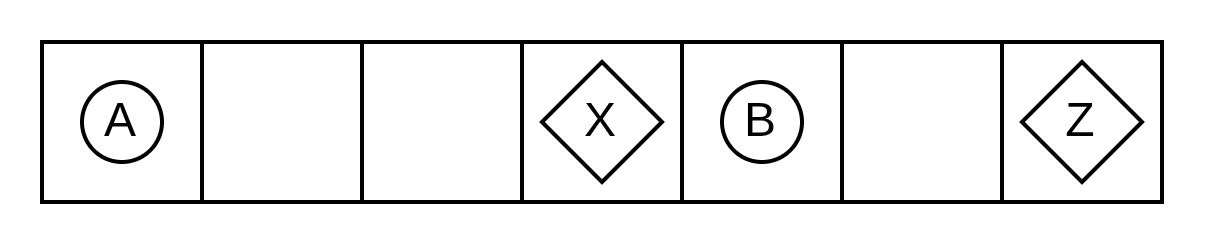
\includegraphics[scale=0.33]{images/task8-impossible}
    \caption{I originally thought this was impossible but it is not}
\end{figure}

    In more complex cases, CBS will usually be able to find a path as long as all nodes are reachable from all nodes and costs are computed optimally.

\section*{Task 9 - Implemented in code}

\section*{Task 10 - }
\begin{table}
    \centering
    \begin{tabular}{llll}
        \toprule
        \textbf{Map} & \textbf{TA-RANDOM} & \textbf{TA-DISTANCE} & \textbf{TA-CBS} \\
        \midrule
        Test 1 & 30, 6/11 & 16, 2/3 & 16, 2/3 \\
        Test 4 & 31, 36/60 & 17, 4/6 & 17, 3/5 \\
        Test 8 & 47, 3118/6004 & 14, 1/1 & 14, 1/1 \\
        \bottomrule
    \end{tabular}
    \caption{(Sum of path lengths), (Num nodes explored)/(Num nodes expanded)}

    All maps except Map 8 using TA-RANDOM were solved in 0.0s, whereas Map 8 took 10.08s.
    The assignment using TA-CBS is optimal in terms of number of nodes expanded and the path cost.
    Since the number of nodes expanded is smaller, the runtime also finished faster!
    In this case, the difference between TA-DISTANCE and TA-CBS is negligible but in cases when the limtations of the hungarian algorithm are met,
    such as if the map is dynamic in nature or a planned allocation ends up changing the map in some way. TA-CBS will be able to deal with these challenges better.
\end{table}

\section*{Task 11}
Since the input paths for the execution come from a CBS run, we are guaranteed that paths are collision free unless a robot has a malfunction.
In a general MAPF setting, assume 2-3 robots share the same path but separated by a sufficient distance k, where a robot visiting a location before another created a predecessor-successor relation.
In this case, even if this path is not a corridor, successive agents might still fail to plan a path successfully around a failed predecessor robot.
They might continue to wait for a robot with a failure, assuming that it will move but it might not.

\section*{Task 12}
\begin{figure}[H]
    \centering
    \includegraphics[scale=0.50]{images/TPG-Rollout.drawio}
    \caption{For each agent R[1-4], the circles denote which vertex they will be at.
    The vertex on the left denotes current time and the vertex on the right is the next location.}
    \label{fig:tpg-rollout.drawio}

    Here we can see that the TPG is cyclic and thus, when attempting to resolve this graph into a sequence of actions for each agent,
    we will not be able to decompose it. Because the TPG has a cycle, it also is a good example of a deadlock!

\end{figure}
\section*{Task 13}
    \begin{table}
        \centering
        \begin{tabular}{ll}
            \toprule
            \textbf{Map} & \textbf{Path-Cost} \\
            \midrule
            Exp\_20 & 33, 358/666 in 2.27s \\
            Exp\_21 & 57, 793/1442 in 8.39s \\
            Exp\_22 & 47, 18/35 in 0.14s \\
            Exp0 & 7, 2/2 in 0.0s \\
            Exp\_2\_2 & 7, 3/5 in 0.0s \\
             &  \\
            \bottomrule
        \end{tabular}
        \caption{}
    \end{table}

\section*{Task 14}
\begin{figure}[H]
    \centering
    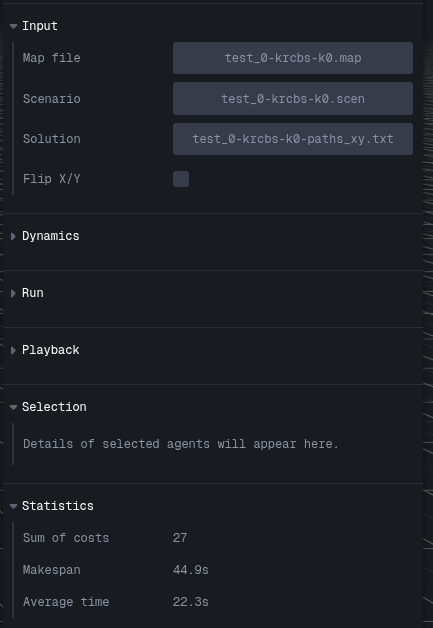
\includegraphics[scale=0.33]{images/Test0_k0_SMART}
    \caption{Output of SMART on Test0 with k=0}
    \label{fig:test0_k0_smart}
\end{figure}

\begin{figure}[H]
    \centering
    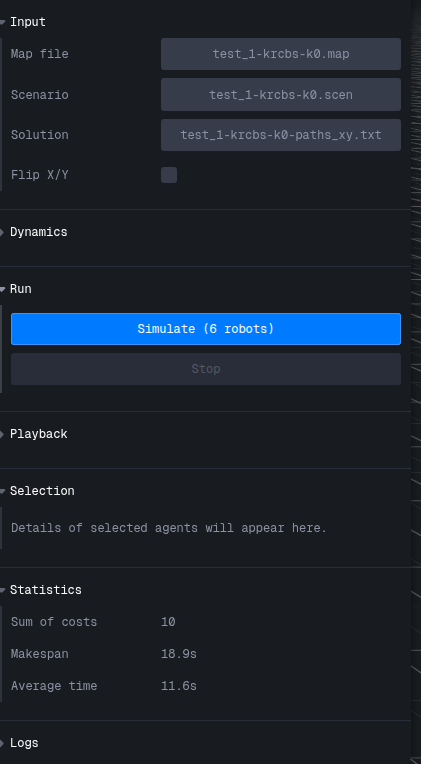
\includegraphics[scale=0.33]{images/Test1_k0_SMART}
    \caption{Output of SMART for Test1 with k=0}
    \label{fig:test1_k0_smart}
\end{figure}

\section*{Task 15}
    The cost reported by the \texttt{sum\_of\_costs} parameter is the sum of the actions taken by each of the agents.
    The action space for both the simulation environments is different - while we have a holonomic robot that can move freely in any direction, the robot in SMART can only rotate in place and move straight.
    This means that to go from point A to B where A is at the bottom of a grid and B is at the top, a holonomic robot will have nearly half the cost of a non holonomic robot like the one in SMART.
    Thus, the costs will differ.

    Since turning is now an action, this means that the robot's position does not change for 2 timesteps every time it rotates,
    meaning the k-robust planning might have to wait for longer or plan for longer to move around other robots, especially if in a bottleneck.
    If the robot has a $p$ probability of failure during execution, this implies it can be stuck along its path with a higher probability.

    All of this follows from the fact that the path is longer now.
\section*{Task 16}
    \begin{lstlisting}
def a_star(my_map, start_loc, goal_loc, h_values, agent, constraints, max_path_length=-1):
    """ my_map      - binary obstacle map
        start_loc   - start position
        goal_loc    - goal position
        h_values    - precomputed heuristic values for each location on the map
        agent       - the agent that is being re-planned
        constraints - constraints defining where robot should or cannot go at each timestep
    """

        #############################
        # Extend the A* search to search in the space-time domain
        #           rather than space domain, only.

        open_list = []
        closed_list = dict()
        earliest_goal_timestep = 0
        prev_goal_timestep = 0
        h_value = h_values[start_loc]
        agent_table = build_constraint_table(constraints, agent)

        # If the start position is forbidden at t=0, no path exists
        if is_constrained(start_loc, start_loc, 0, agent_table):
            return None, float('inf')
        root = {'loc': start_loc,
                'g_val': 0,
                'h_val': h_value,
                'parent': None,
                "timestep": 0}

        push_node(open_list, root)
        closed_list[(root['loc'], root["timestep"])] = root

        while len(open_list) > 0:
            curr = pop_node(open_list)

            if max_path_length != -1 and curr["timestep"] > max_path_length:
                return None, float('inf')

            #############################
            # Task 2.2: Adjust the goal test condition to handle goal constraints
            if curr['loc'] == goal_loc:
                prev_goal_timestep = curr["timestep"]
                can_stop = True
                for k in agent_table.keys():
                    if k > prev_goal_timestep:
                        can_stop = False
                        break

                if can_stop:
                    return get_path(curr), curr["g_val"]  (*@\textbf{\textcolor{blue}{$\leftarrow$}}@*)

            for dir in range(len(directions)):
                child_loc = move(curr['loc'], dir)
                if (not in_map(my_map, child_loc) or
                        my_map[child_loc[0]][child_loc[1]] or
                        is_constrained(curr["loc"], child_loc, curr["timestep"] + 1,
                                       agent_table)):
                    continue

                child = {'loc': child_loc,
                         'g_val': curr['g_val'] + 1,
                         'h_val': h_values[child_loc],
                         'parent': curr,
                         "timestep": curr["timestep"] + 1}

                ### To match the costs of the SMART simulator!
                child["g_val"] = increase_cost_2(child)  (*@\textbf{\textcolor{blue}{$\leftarrow$}}@*)
                #############################################

                if (child['loc'], child["timestep"]) in closed_list:
                    existing_node = closed_list[(child['loc'], child["timestep"])]
                    if compare_nodes(child, existing_node):
                        closed_list[(child['loc'], child["timestep"])] = child
                        push_node(open_list, child)
                else:
                    closed_list[(child['loc'], child["timestep"])] = child
                    push_node(open_list, child)

        return None, float('inf')
    \end{lstlisting}

    \begin{lstlisting}
def increase_cost_2(node: Dict) -> int:
    cost_increase = 0
    if node['g_val'] > 1:
        prev_prev_loc = node["parent"]["parent"]["loc"]
        prev_loc = node["parent"]["loc"]
        curr_loc = node["loc"]

        p2p_action = (prev_prev_loc[0] - prev_loc[0], prev_prev_loc[1] - prev_loc[1])  (*@\textbf{\textcolor{blue}{$\leftarrow$}}@*)
        p2c_action = (prev_loc[0] - curr_loc[0], prev_loc[1] - curr_loc[1])            (*@\textbf{\textcolor{blue}{$\leftarrow$}}@*)

        if p2p_action != p2c_action:
            cost_increase += 1

    return node["g_val"] + cost_increase
    \end{lstlisting}

\begin{table}
    \centering
    \begin{tabular}{lll}
        \toprule
        \textbf{Map Name} & \textbf{Previous Cost } & \textbf{Modified Algorithm Cost} \\
        \midrule
        Exp0, k1 - Python & 7, 2/2 in 0s &  \\
        Exp0 - SMART &  &  \\
        Exp2\_2 - Python & 7, 3/5 in 0.0s &  \\
        Exp2\_2 - SMART &  &  \\
        Test 20, k1 - Python & 33, 358/666 in 2.2s &  \\
        Test 20 - SMART &  &  \\
        Test 21, k1 - Python & 57, 793/1442 in 8.3s &  \\
        Test 21 - SMART &  &  \\
        Test 22, k1 - Python & 47, 18/35 in 0.1s &  \\
        Test 22 - SMART &  &  \\
        \bottomrule
    \end{tabular}
    \caption{}
    \label{tab:}
\end{table}

\section*{Task 17}

\end{document} % Done!
